\documentclass[slidestop,compress,mathserif]{beamer}
\usetheme{Frankfurt}
\usecolortheme{seagull}
\definecolor{links}{HTML}{2A1B81}
\hypersetup{colorlinks,linkcolor=,urlcolor=links}

% Load packages
\usepackage{alltt}
\usepackage{verbatim}
\usepackage{geometry}                % See geometry.pdf to learn the layout options. There are lots.
\usepackage{graphicx}
\usepackage{amssymb}
\usepackage{amsmath}
\usepackage{epstopdf}
\usepackage{verbatim}
%\usepackage{musixtex}
%\usepackage{xymtexps}
\usepackage{feynmp}

%\usepackage{pgfpages}
%\pgfpagesuselayout{4 on 1}[letterpaper,landscape,border shrink=5mm]

\DeclareGraphicsRule{.tif}{png}{.png}{`convert #1 `dirname #1`/`basename #1 .tif`.png}


% Title 
% Note: [short title]{long title}, [short author(s) name]{long author(s) name}
\title{Math and LaTeX}
\subtitle{}
\author{Viktor Dmitriyev} 
\institute{Adapter from Mini Course on LaTeX by \href{https://github.com/OpenIntroOrg/mini-course-materials}{David Diez}}
\date{}

\begin{document}
\definecolor{highlight}{rgb}{.7,.1,.1}
\definecolor{command}{rgb}{.1,.1,.9}
\definecolor{comment}{rgb}{1,0,0}
\definecolor{braces}{rgb}{0,0.5,0}
\newenvironment{act}[1]{{\color{command}#1}}{}
\newcommand{\lcom}[1]{{\color{command}$\backslash$#1}}
\newcommand{\larg}[1]{{\color{braces}$\{${\color{black}#1}$\}$}}
\newcommand{\mathText}[1]{{\color{braces}\${\color{black}#1}\$}}


\frame{ \titlepage }

\begin{frame}
  \frametitle{Outline}
  \begin{itemize}
	  \item Mathematics in LaTeX
  \end{itemize}
\end{frame}

\part{}


%READ ME
% two new commands were created to ease LaTeX command appearance.
%    use \lcom{command} to print a command, which includes coloring and the backslash
%    use \larg{argument} to print an argument in green braces
%    use \mathText{math text} to print an argument with two green $ around it
% additionally, combine the commands:
%    \mathText{\lcom{alpha}}
%    instead of 
%    {\color{braces}\$}\texttt{\color{command}$\backslash$alpha}\texttt{\color{braces}\$}

\section[Math]{Math}

\subsection[Mathematics]{Mathematics}
\begin{frame} \frametitle{Math in LaTeX}
We will cover several aspects of the mathematics environments offered in LaTeX.
\begin{itemize}
\item Basic mathematics in text
\item Different equation environments
\item Mathematical symbols
\item Mathematical expressions
\item Accenting and modifying text
\item Automatic sizing of bracket symbols
\item Text in mathematical equations
\item Arrays and matrices
\end{itemize}
\end{frame}

\subsection[Inserting math]{Inserting math}
\begin{frame} \frametitle{Inserting math into text}
LaTeX makes it easy to add Greek letters like $\alpha$, $\zeta$,
$\mu$, etc. into text. In the same way, equations can be added
easily as well: $y=x^3$, $\sum z^j$, $x_1+\cdots+x_n$.
\begin{center}
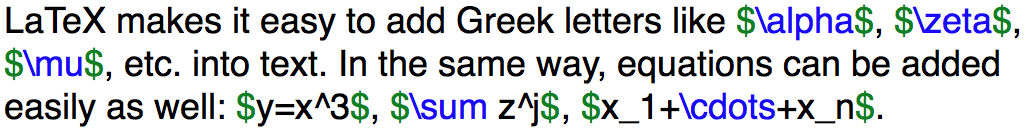
\includegraphics[height=0.47in]{math/mathInText}
\end{center}
The {\color{braces}\$} signs tell LaTeX when to switch into or out of math model. For instance, to create $\alpha$ above, type \mathText{\lcom{alpha}}. %{\color{braces}\$}\texttt{\color{command}$\backslash$alpha}\texttt{\color{braces}\$}.
\vspace{5mm} \\
How can we create $\beta$?
\end{frame}

\begin{frame} \frametitle{Equation array}
Some equations are long and should be on their on lines. In such a case, use the \texttt{\color{highlight}eqnarray} or \texttt{\color{highlight}eqnarray$^*$} environment:
\begin{center}
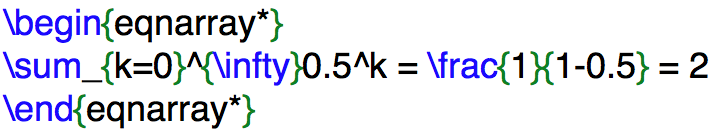
\includegraphics[height=0.4in]{math/eqnarrayStar}
\end{center}
The result in LaTeX for \texttt{\color{highlight}eqnarray$^*$}:
\begin{eqnarray*}
\sum_{k=0}^{\infty}0.5^k = \frac{1}{1-0.5} = 2
\end{eqnarray*}
\end{frame}

\begin{frame} \frametitle{Equation referencing}
Just like tables and figures, equations can be referenced. Use \texttt{\color{highlight}eqnarray} (no asterisk) to add an equation number:
\begin{eqnarray}
\sum_{k=0}^{\infty}0.5^k = \frac{1}{1-0.5} = 2
\end{eqnarray}
\texttt{\color{command}$\backslash$label}\texttt{\color{braces}\{}\texttt{powerSeries}\texttt{\color{braces}\}} can be put inside the equation array and then be referenced via \texttt{\color{command}$\backslash$ref}\texttt{\color{braces}\{}\texttt{powerSeries}\texttt{\color{braces}\}}.
\begin{center}
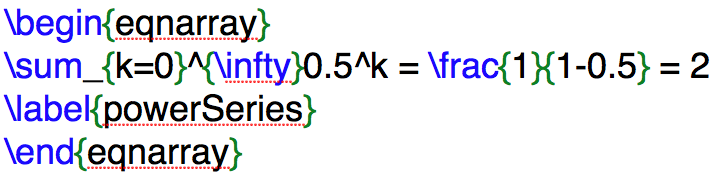
\includegraphics[height=0.6in]{math/eqnarray}
\end{center}
\end{frame}

\begin{frame} \frametitle{Aligned equations}
Another environment, \texttt{\color{highlight}align} (and \texttt{\color{highlight}align$^*$}) are handy for aligning multiline equations.
\begin{center}
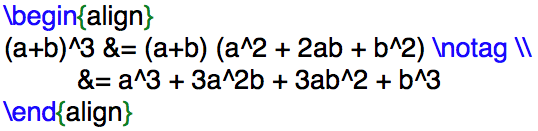
\includegraphics[height=14mm]{math/align}
\end{center}
Result:
\begin{align}
(a+b)^3 &= (a+b) (a^2 + 2ab + b^2) \notag \\
	      &= a^3 + 3a^2b + 3ab^2 + b^3
\end{align}
The \texttt{\color{command}$\backslash\backslash$} command creates a line break. The command \texttt{\color{command}$\backslash$notag} was used to suppress the equation number of the first line, which requires the \texttt{\color{highlight}amsmath} package. (Q: We have an equation number. What should I have included in the code?)
\end{frame}

\begin{frame} \frametitle{Multiple alignments}
The \texttt{\color{highlight}align} environment permits several alignments:
\begin{center}
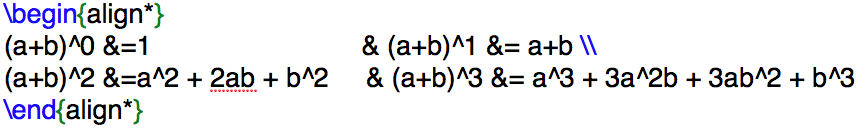
\includegraphics[height=14mm]{math/alignMany}
\end{center}
outputs
\begin{align*}
(a+b)^0 &=1                            & (a+b)^1 &= a+b \\
(a+b)^2 &=a^2 + 2ab + b^2     & (a+b)^3 &= a^3 + 3a^2b + 3ab^2 + b^3
\end{align*}
%The \texttt{\color{command}$\backslash\backslash$} command creates a line break. The command \texttt{\color{command}$\backslash$notag} was used to suppress the equation number of the first line (package \texttt{\color{highlight}amsmath} required).
%\texttt{\color{command}$\backslash$label}\texttt{\color{braces}\{}\texttt{powerSeries}\texttt{\color{braces}\}} can be put inside the equation array and then be referenced via \texttt{\color{command}$\backslash$ref}\texttt{\color{braces}\{}\texttt{powerSeries}\texttt{\color{braces}\}}.
\end{frame}

\subsection[Mathematics and symbols]{Mathematics and symbols}

\begin{frame} \frametitle{Mathematics and symbols}
It is a little difficult to learn all the math syntax and a good help source is the LaTeX and Matrix Panels:
\begin{center}
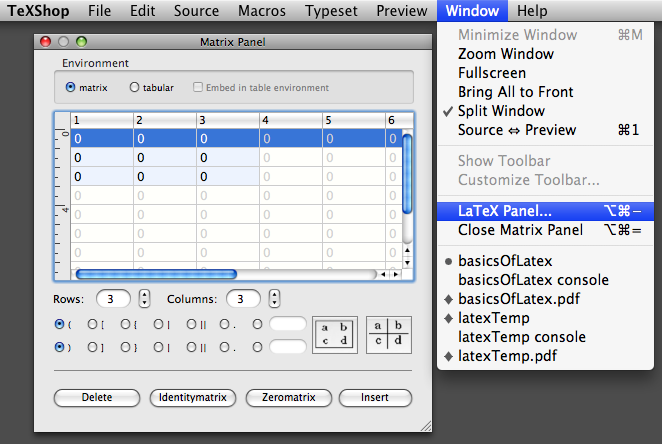
\includegraphics[height=1.5in]{math/panels}
\end{center}
The Matrix Panel is especially useful since matrices can require a lot of writing. The LaTeX panel is handy as a quick reference.
\end{frame}

\begin{frame} \frametitle{Some symbols}
Here is a very small subset of the symbols available in LaTeX.
%\begin{center}
\begin{tabular}{rl p{4mm} rl p{4mm} rl}
$\leftarrow$ & {\color{braces}\${\color{command}$\backslash$leftarrow}\$} &&
$\Leftarrow$ & {\color{braces}\${\color{command}$\backslash$Leftarrow}\$} && 
$\leftrightarrow$ & {\color{braces}\${\color{command}$\backslash$leftrightarrow}\$} \\
$\geq$ & {\color{braces}\${\color{command}$\backslash$geq}\$} &&
$\neq$ & {\color{braces}\${\color{command}$\backslash$neq}\$} &&
$\not\in$ & {\color{braces}\${\color{command}$\backslash$not$\backslash$in}\$} \\
$\partial$ & {\color{braces}\${\color{command}$\backslash$partial}\$} &&
$\oint$ & {\color{braces}\${\color{command}$\backslash$oint}\$} &&
$\nabla$ & {\color{braces}\${\color{command}$\backslash$nabla}\$} \\
$\bigcap$ & {\color{braces}\${\color{command}$\backslash$bigcap}\$} &&
$\bigcup$ & {\color{braces}\${\color{command}$\backslash$bigcup}\$} &&
$\cap$ & {\color{braces}\${\color{command}$\backslash$cap}\$} \\
$\subset$ & {\color{braces}\${\color{command}$\backslash$subset}\$} &&
$\supseteq$ & {\color{braces}\${\color{command}$\backslash$supseteq}\$} &&
$\not\supseteq$ & {\color{braces}\${\color{command}$\backslash$not$\backslash$supseteq}\$} \\
$\bigodot$ & {\color{braces}\${\color{command}$\backslash$bigodot}\$} &&
$\bigotimes$ & {\color{braces}\${\color{command}$\backslash$bigotimes}\$} &&
$\oplus$ & {\color{braces}\${\color{command}$\backslash$oplus}\$} \\
$\clubsuit$ & {\color{braces}\${\color{command}$\backslash$clubsuit}\$} &&
$\perp$ & {\color{braces}\${\color{command}$\backslash$perp}\$} &&
$\vdash$ & {\color{braces}\${\color{command}$\backslash$vdash}\$} \\
\end{tabular}
%\end{center}
For a searchable PDF with thousands of symbols, see
\begin{itemize}
\item[] {\small\color{highlight}www.ctan.org/tex-archive/info/symbols/comprehensive/symbols-a4.pdf}
\end{itemize}
Also see the LaTeX Panel (under the menu item {\color{highlight}Window}).
\end{frame}

\begin{frame} \frametitle{Character modifications}
Text and symbols in math mode can also be modified.
\begin{center}
\begin{tabular}{rl p{4mm} rl p{4mm} rl}
\hline
\multicolumn{3}{l}{Regular} & {Modified} &&& {Accents} & \\
\hline
{\color{braces}\${\color{black}R}\$} & $R$ &&
{\color{braces}\${\color{command}$\backslash$mathbb}$\{${\color{black}R}$\}$\$} & $\mathbb{R}$ &&
{\color{braces}\${\color{command}$\backslash$tilde}$\{${\color{black}R}$\}$\$} & $\tilde{R}$ \\
{\color{braces}\${\color{black}A}\$} & $A$ &&
{\color{braces}\${\color{command}$\backslash$mathcal}$\{${\color{black}A}$\}$\$} & $\mathcal{A}$ &&
{\color{braces}\${\color{command}$\backslash$widetilde}$\{${\color{black}A}$\}$\$} & $\widetilde{A}$ \\
{\color{braces}\${\color{black}x}\$} & $x$ &&
{\color{braces}\${\color{command}$\backslash$mathbf}$\{${\color{black}x}$\}$\$} & $\mathbf{x}$ &&
{\color{braces}\${\color{command}$\backslash$bar}$\{${\color{black}x}$\}$\$} & $\bar{x}$ \\
{\color{braces}\${\color{black}p}\$} & $p$ &&
{\color{braces}\${\color{command}$\backslash$mathit}$\{${\color{black}p}$\}$\$} & $\mathit{p}$ &&
{\color{braces}\${\color{command}$\backslash$hat}$\{${\color{black}p}$\}$\$} & $\hat{p}$ \\
{\color{braces}\${\color{black}X}\$} & $X$ &&
{\color{braces}\${\color{command}$\backslash$mathrm}$\{${\color{black}X}$\}$\$} & $\mathrm{X}$ &&
{\color{braces}\${\color{command}$\backslash$widehat}$\{${\color{black}X}$\}$\$} & $\widehat{X}$ \\
\hline
\end{tabular}
\end{center}
Two other accents: $\dot{x}$ and $\ddot{x}$ via {\color{braces}\${\color{command}$\backslash$dot}$\{${\color{black}x}$\}$\$} and {\color{braces}\${\color{command}$\backslash$ddot}$\{${\color{black}x}$\}$\$}.
\end{frame}

\begin{frame} \frametitle{Subscripts and exponents}
We can create subscripts (e.g. $x_1$) and superscripts (e.g. $3^2$):
\begin{center}

\includegraphics[height=8mm]{math/subSuperscript}
\end{center}
When the subscript is a single character, then it is acceptable to omit the curly braces. That is, the following is equally acceptable for the text above:
\begin{center}

\includegraphics[height=8mm]{math/subSuperscriptNoBraces}
\end{center}
If more than one character is in the sub/superscript, braces are necessary to avoid problems: {\color{braces}\${\color{black}2\textbf{\_}10}\$} outputs $2_10$. Sub and superscripts can be used simultaneously: $x_{ij}^2$.
\end{frame}

\begin{frame} \frametitle{Fractions and roots}
We can easily create fractions such as $\frac{2+3}{4+5} = \frac{5}{9}$ or roots such as $\sqrt{81}=9$ and $\sqrt[4]{81} = 3$.
\begin{center}
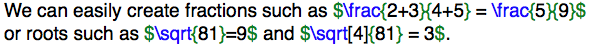
\includegraphics[height=7mm]{math/fracRoots}
\end{center}
And we can combine them as well:
$\frac{\sqrt{4} + 3}{\sqrt{16} + 5} = \frac{5}{9}$.
\begin{center}
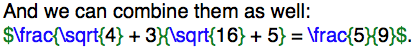
\includegraphics[height=7mm]{math/fracRootsCombined}
\end{center}
\end{frame}

\begin{frame} \frametitle{Sums and integrals}
We can also create sums and integrals:
\begin{center}
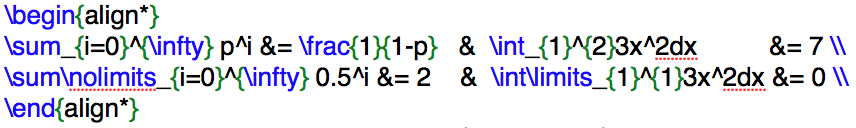
\includegraphics[height=14mm]{math/sumIntegral}
\end{center}
which results in
\begin{align*}
\sum_{i=0}^{\infty} p^i &= \frac{1}{1-p}   &  \int_{1}^{2}3x^2dx          &= 7 \\
\sum\nolimits_{i=0}^{\infty} 0.5^i &= 2    &  \int\limits_{1}^{1}3x^2dx &= 0
\end{align*}
The commands \texttt{\color{command}$\backslash$nolimits} and \texttt{\color{command}$\backslash$limits} can be used to override the default displays of limits in LaTeX.
\end{frame}

\begin{frame} \frametitle{Practice}
Produce the following result using the \texttt{\color{highlight}eqnarray$^*$} environment:
\begin{center}
   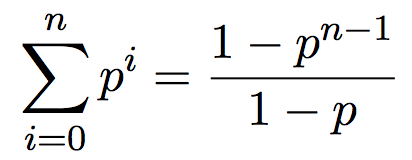
\includegraphics[height=0.6in]{math/tryIt3}
\end{center}
Some examples may be utilized in \texttt{\color{highlight}latexTemp.tex}.
\end{frame}

\subsection[Final items]{Final items}
\begin{frame} \frametitle{Sizing of Brackets}
A small problem with bracket sizes is shown in the left equation, and this problem is fixed on the right.
\begin{align*}
   (\frac{2+3}{4+5}) &&& \left(\frac{2+3}{4+5}\right)
\end{align*}
The coding for the expressions above 
\begin{center}
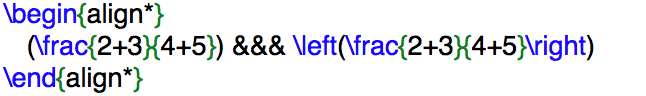
\includegraphics[height=9mm]{math/fixingParentheses}
\end{center}
Generally we can use {\color{command}$\backslash$left\color{black}(}, {\color{command}$\backslash$left\color{black}[}, {\color{command}$\backslash$left\color{black}$|$}, and {\color{command}$\backslash$left$\backslash\{$} and their corresponding right brackets to create automatically sized brackets. These commands \emph{must} be inside one of the equations environments and the left and right brackets must always be balanced.
\end{frame}

\begin{frame} \frametitle{Matrices}
Matrices also can be made in LaTeX:
\begin{eqnarray*}
\left(\begin{array}{ccc} 4 & 1 & 19 \\ 3 & 8 & 8\end{array}\right)
\end{eqnarray*}
The code:
\begin{center}
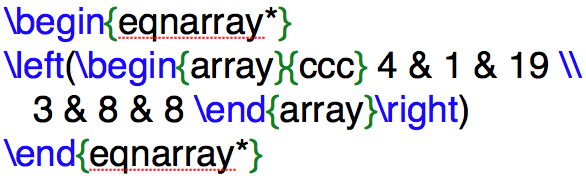
\includegraphics[height=0.6in]{math/array}
\end{center}
The syntax for an \texttt{\color{highlight}array} is the same as for \texttt{\color{highlight}tabular} (a table).
\end{frame}

\begin{frame} \frametitle{Space and stacking}
Space can be added in equations using {\color{command}$\backslash$quad}, and expressions can be stacked via {\color{command}$\backslash$stackrel}:

\vspace{1mm}

\begin{itemize}
\item[] {\color{command}$\backslash$begin}{\color{braces}$\{${\color{black}eqnarray$^*$}$\}$}
\item[] \hspace{2mm} E(X+Y)
	{\color{command}$\backslash$stackrel\color{braces}$\{${\color{black}indep.}$\}\{${\color{black}=}$\}$}
	E(X) + E(Y)
\item[] \hspace{5mm} {\color{command}$\backslash$quad$\backslash$quad}
\item[] \hspace{5mm} Var(X+Y)
	{\color{command}$\backslash$stackrel\color{braces}$\{${\color{black}indep.}$\}\{${\color{black}=}$\}$}
	Var(X) + Var(Y)
\item[] {\color{command}$\backslash$end}{\color{braces}$\{${\color{black}eqnarray$^*$}$\}$}
\end{itemize}

\vspace{1mm}

produces
\begin{eqnarray*}
E(X+Y) \stackrel{indep.}{=} E(X) + E(Y) \quad\quad Var(X+Y) \stackrel{indep.}{=} Var(X) + Var(Y)
\end{eqnarray*}
\end{frame}



\section[Summary]{Summary}
\subsection[Summary]{Summary}

\begin{frame}  \frametitle{Summary}
After this class, you should have a general idea of
	\vspace{1mm} \\
		\begin{itemize}
			\item using the math modes in LaTeX
		\end{itemize}
	\vspace{1mm}

Any questions?
\end{frame}





\end{document}